\documentclass{template/openetcs_article}
%\documentclass{article}
%\usepackage[ascii]{inputenc}
%\usepackage[T1]{fontenc}
\usepackage[english]{babel}
\usepackage{amsmath}
\usepackage{amssymb,amsfonts,textcomp}
\usepackage{array}
\usepackage{supertabular}
\usepackage{hhline}
\usepackage{graphicx}
\makeatletter
\newcommand\arraybslash{\let\\\@arraycr}
\makeatother
\setlength\tabcolsep{1mm}
\renewcommand\arraystretch{1.3}
\newcounter{Ilustracin}
\renewcommand\theIlustracin{\arabic{Ilustracin}}
\title{openETCS}

%\setcounter{tocdepth}{3}
\usepackage{float}
\usepackage{hhline}
\usepackage{booktabs}
\usepackage{multirow}
\usepackage{color, colortbl}
\definecolor{myblue}{rgb}{0.6,.6,1}
\definecolor{mydarkblue}{rgb}{0,0,0.5}
\definecolor{mylightblue}{rgb}{0.8,0.8,1}
\usepackage{hyperref}
\hypersetup{colorlinks=true, linkcolor=mydarkblue, urlcolor=mydarkblue}

\usepackage[textwidth=2.7cm,textsize=scriptsize,linecolor=green!40,backgroundcolor=green!40]{todonotes}

\newcounter{mycommentcounter}
\newcommand{\mycomment}[2][]
{
\refstepcounter{mycommentcounter}%
\todo[color={red!100!green!33}]{
\textbf{[\uppercase{#1} \themycommentcounter]:} #2}
}


\usepackage{lipsum,url}
\graphicspath{{./template/}{.}{./images/}}
\begin{document}
\frontmatter
\project{openETCS}

%Please do not change anything above this line
%============================
% The document metadata is defined below

%assign a report number here
\reportnum{OETCS/WP1/D1.3.1}

%define your workpackage here
\wp{Work-Package 1: ``Management''}

%set a title here
\title{Project Quality Assurance Plan - Review Process}

%set a subtitle here
%\subtitle{A template for short document. Adapted from report template.}

%set the date of the report here
\date{\today}

%define a list of authors and their affiliation here

\author{Ainhoa Gracia}

\affiliation{Avda. Zugazarte 8,6\\
  48930 Getxo \\
  Vizcaya, España}


% define the coverart
\coverart[width=350pt]{openETCS_EUPL}

%define the type of report
\reporttype{Description of work}




%=============================
%Do not change the next three lines
\maketitle
\tableofcontents
%\listoffiguresandtables
\newpage
%=============================

% The actual document starts below this line
%=============================


%Start here



%\begin{document}


\section*{Document History}

\begin{flushleft}
%\tablefirsthead{\hline Version & Date & Chapters modified & Reason & Name\\}

\tablehead{\hline \rowcolor{myblue} Version & Date & Chapters modified & Reason & Name\\}

\tabletail{}
\tablelasttail{}
\begin{supertabular}{m{1.1cm}m{1.8cm}m{2cm}m{7cm}m{2cm}lp{6cm}|}
\hline
0.0.1 &
24.05.2013 &
All &
First version &
SQS
\end{supertabular}
\end{flushleft}

\newpage

\section{Introduction}

\subsection[Introduction]{Purpose of the document}
This document presents the whole process to follow when documents need review. It aims to provide a set of guidelines as technical instructions to be used whenever a review process is ongoing, or there are a set of issues reported that shall be considered. The roles involved in the process are clearly identified as well as their responsibilities and tasks. And finally, the mechanisms needed to achieve the proposed objectives are also included, so the process can be carried out successfully.

\subsection{Intended Audience}
This document applies to the whole development life-cycle of the project and it addresses all the author(s)and reviewers involved. This document should be available to all of them in read access mode and it provides guidance about the Review process whenever it is needed. 

\subsection{Supporting documents}
\tablefirsthead{\hline
\rowcolor{myblue}
Name &
Path &
Contents\\}
\tablehead{}
\tabletail{}
\tablelasttail{}
\begin{supertabular}{|m{2cm}m{3cm}m{9cm}|}
\hline
Revision process &
governance/Review Process &
Presentation of the Revision process with details about the flow and technical instructions.
\\\hline
Revision and Review Processes summary &
governance/Review Process &
Brief presentation of the Revision process and the Review process as well as their interactions.
\\\hline
Review Guidelines &
Governance/ecosystem &
It describes major aspects to be assessed during a Review Cycle.
\\\hline
\end{supertabular}

\subsection{Definitions and acronyms}
\tablefirsthead{\hline
\rowcolor{myblue}
Abbreviation &
Meaning\\}
\tablehead{}
\tabletail{}
\tablelasttail{}
\begin{supertabular}{|m{3cm}m{11cm}|}
\hline
Revision Process &
The OpenETCS committers are invited to perform a revision of the contents of a document. The committers can edit the document, writing complete sections or making changes directly in it (LaTex, todonotes and Smartgit tools). The author(s) shall support the whole process answering questions and resolving conflicts. Once the author(s) and committers are satisfied with the results, the Product owner shall confirm and approve or reject and request more changes to the revised document. Finally, the approved document is pushed into the corresponding GitHub repository.
\\\hline
Committer &
The role played by a member of the OpenETCS project who have been granted with this role by other committers and the project leader. There are some tasks that only can be done by committers such as: editing and pushing changes or new documents into a GitHub repository, closing of issues in the {\it Issue Tracker} or being involved in Revision processes.
\\\hline
\end{supertabular}

\section{Tools}

\begin{flushleft}

\begin{tabular}{|m{3cm}|m{11cm}|}
\hline
\rowcolor{myblue}
\multicolumn{2}{|c|}{Tools} \\\hline
GIT &
\begin{itemize}
\item \underline{GitHub}: A web-based hosting service for projects that use Git revision control system.
\item \underline{Issue Tracker (in GitHub)}: The issue tracker is integrated with the project's repository. Some of the features included are: the possibility of modifying tickets from within commit messages,
creating and applying labels to issues to assign to users or categorize, voting on issues that you want to see tackled, searching, sorting, and filtering, and keyboard shortcuts.
\end{itemize}
\\\hline
PDF documents &
\begin{itemize}
\item \underline{Adobe Acrobat Reader}: Software package that allows to view, navigate and print pdf files.
\item \underline{Diffpdf}: Open source application that compares different PDF files for discrepancies. 
\end{itemize}
\\\hline
\end{tabular}
\end{flushleft}

\section{Review Process overview}

There are two types of Review Processes:
\begin{itemize}
\item Planned Review Process: It is launched by the product owner; there is a deadline for receiving comments (by default, 2 weeks) from the community and if considered appropriate, there are well identified review objectives and/or guidelines. A Planned Review Process will always be launched after a Revision Process.
\item Open Review Process: At any time, an expert can make comments and suggest improvements to the documents published in the repository. Comments will be assessed by the Product Owner as they are received, and the appropriate actions taken.
\end{itemize}

In both cases:
\begin{itemize}
\item The review process will be performed against documents already revised and therefore published in the repository. Therefore no specific branch for review will be created.
\item All comments will be made and answered using the Issue Tracker tool.
\item The Product Owner will be assisted by a group of selected Key Customers of the document under review when necessary.
\end{itemize}

\subsection{Structure of the repository}
 
There is no need of additional working directories for a Review process, considering no branches shall be created and the changes to be included in a version of a document shall be minor changes.

\subsection{Review Roles}

This section describes the roles of the participants in the review process of a document:

\begin{flushleft}
\begin{tabular}{|m{3cm}|m{11cm}|}
\hline
\rowcolor{myblue}
\multicolumn{2}{|c|}{Roles} \\\hline
\rowcolor{lightgray}
Role &
Competencies \\\hline
Product owner &
He/She is the main responsible of a document. He/She is in charge of launching the review; preparing the plan and controlling and monitoring the process progresses according to the plan; informing and interacting with the review team members \\\hline
Review Team &
As experts in the theme of the project, they will provide meaningful contributions to guarantee the document meets its scope and purpose in a complete and accurate way.\\\hline
Key Customers  &
It is composed of members of the community of users of a document. Their role is to guarantee completeness, accuracy and validity of the contents of a document. Therefore, they are not only reviewers but they will assess the Product Owner in the acceptance for publication of a document. \\\hline
\end{tabular}
\end{flushleft}


\subsection{Description of the Review Process}

The next figure shows the different stages of the Review Process. Right after the activities to be performed in each Stage are provided. The technical instructions on how to accomplish such activities are included in the Annex.

\begin{figure}[H]
\centering
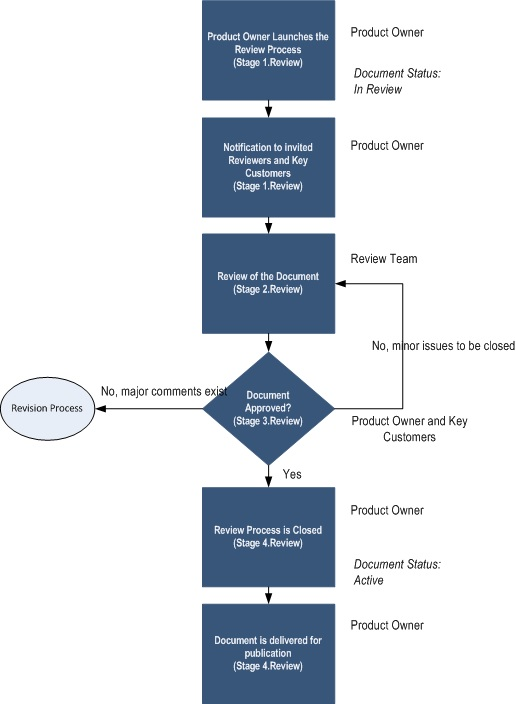
\includegraphics{./figures/Review_Process.JPG}
\caption{Review Process flow}
\end{figure}


\subsubsection{Stage One: Launching of the Review Process}

\begin{itemize}
\item The Product Owner elaborates the Review Plan with the information to be sent to the reviewers: deadline for the different stages and specific review guidelines and/or objectives.
\item The Product Owner updates the status of the document in wiki to “In Review”. 
\item The Product Owner creates the list of reviewers and key customers and invites them to participate. Refer to {\it A2.Review Process-Control and Monitoring} in Annex for Technical Instructions.
\item The Review Process is officially launched.
\end{itemize}

\subsubsection{Stage Two: The Review Process}

\begin{itemize}
\item Reviewers will make comments in the form of appropriately labeled Issues. Reviewers are invited to include the “relevance” of the comment (high, medium, low). Refer to Section {\it A3. Review Process} for detailed instructions.
\item The Product Owner jointly with the Authors will interact with the reviewers, when needed, in order to clarify comments.  
\item The deadline for receiving comments may be extended by the Product Owner. Both the finalization and the extension will be notified to the revision team members. Refer to {\it A2.Review Process-Control and Monitoring} in Annex for Technical Instructions.
\end{itemize}

\subsubsection{Stage Three: The Approval Process}

\begin{itemize}
\item The Product Owner will analyze the comments and proceed with their acceptance or rejection. In case of conflicts, the Key Customers will support the Product Owner in this process. Refer to {\it A4.Approval/Rejection of changes} in Annex for Technical Instructions.
\item The Product Owner will implement the changes in the document under review.  
\item The Product Owner with the support of the Key Customer will decide whether the project is ready for publication or not.
\item If ready for publication, the review process will be closed. Otherwise, a revision process will be launched, A notification with the published in the form of an issue. Refer to {\it A2.Review Process-Control and Monitoring} in Annex for Technical Instructions.
\end{itemize}

\subsubsection{Stage Four: Review Closing}

\begin{itemize}
\item The Product Owner publishes a new version of the document. Refer to section {\it A12.Versioning} for versioning instructions.
\item The Product Owner closes the Review Process. Refer to section {\it A6. Review Closing} for instructions 
\item The Product Owner updates the status of the document in the wiki of the Project to “Active”.
\end{itemize}

\section{ANNEXES - Technical Instructions for using the Issue Tracker tool}

\textbf{A2. Review Process-Control and Monitoring}

\begin{flushleft}
\tablefirsthead{}
\tablehead{}
\tabletail{}
\tablelasttail{}
\begin{supertabular}{|m{3cm}|m{12cm}|}
\hline
\rowcolor{myblue}
TI & 
Review Process-Control and Monitoring
\\\hline
\rowcolor{lightgray}
Action &
Role/Instruction
\\\hline
Invitation to Participate to the Review Team &
\begin{description}
\item Product Owner\
\item Create a new Issue (Main Issue of the Review Process) in the Repository indicating a new review is launched:
\begin{itemize}
\item Open Github and go to the correspondent repository
\item Select the {\it Issues section}
\item Push the {\it New issue} button
\item Add a descriptive title indicating the document under review
\item Add a significant description about the causes that have motivated the review and summarizes the objectives of the review. Provide the list of required Committers/Contributors.
\item Push {\it Submit new issue} 
\end{itemize}
\item Besides, a direct mail addressing the selected Review Team Members will be sent.
\end{description} 
\\\hline
Interaction with the Review Team to clarify comments &
\begin{description}
\item Product Owner\
\item Create an Issue addressing the corresponding Review Team Member:
\begin{itemize}
\item Add a Title identifying the RC process
\item Add Text describing the details of the clarification requested
\end{itemize}
\item This Issue will be the Main Issue for the interaction with the expert. The rest of the communication will adopt the form of Comments to this Main Issue
\end{description}
\\\hline
Notification of Extension of the Review Stage &
\begin{description}
\item Product Owner\
\item Add a Comment to the Main Issue of the Review Process indicating the deadline for receiving comments has been extended. The new deadline will be indicated.
\end{description}\\\hline
Notification that the Review Stage has finalized &
\begin{description}
\item Product Owner\
\item Add a Comment to the Main Issue of the Review Process indicating the date for receiving comments has finalized.
\end{description} 
\\\hline
\end{supertabular}
\end{flushleft}

\textbf{A3. Review Process}

\begin{flushleft}
\tablefirsthead{}
\tablehead{}
\tabletail{}
\tablelasttail{}
\begin{supertabular}{|m{2cm}|m{13cm}|}
\hline
\rowcolor{myblue}
TI & 
Review work
\\\hline
Roles &
Review Team
\\\hline
Description &
The review team shall perform the review in the expected time and conditions. The work of the review team shall finish when the Product owner confirms the closing of the Review Process.
\\\hline
Steps &
The reviewers shall:
\begin{enumerate}
\item Make comments, suggestions or improvement proposals with the {\it Issue Tracker tool}.
\item Add comments in the Rewiew issue thread when it applies:
\begin{itemize}
\item Go to the repository where the document under Review is located.
\item Select the issue that refers to the document under Review.
\item The reviewers comments posted shall be a reference to a new issue (if it not exists) where a description of the comments, suggestions or improvement proposal is.
\item Push the {\it Comment} button to post the message.
\item Create a new issue in the repository that contains the document under review. 
\begin{enumerate}
\item Open Github and go to the appropriate repository
\item Select the {\it Issues section}
\item Push the {\it New issue} button
\item Add a descriptive title indicating the name of Document under Review and a brief title for the comment/suggestion or improvement
\item Provide descriptive enough so any reader can understand the message.
\item When required, include diagrams, figures, partial texts or specific data that help to understand the problematic found.
\item Push Submit new issue
\end{enumerate}
\item If a issue exists regarding to the same aspects you want proposed for the document under review, post a reference to the existing review issue, and in the corresponding issue add a comment. Do not edit any comment done. Add a new comment with the additions you proposed.
\item Push the {\it Comment} button to post the message.
\end{itemize}
\end{enumerate}
\\\hline
Steps &
\begin{itemize}
\item In any case, the reviewers shall inform about the progress of the work posting a message in the Review issue thread or sending an e-mail. 
\end{itemize}
\\\hline
\end{supertabular}
\end{flushleft}

\textbf{A4. Approval/Rejection of Changes}

\begin{flushleft}
\tablefirsthead{}
\tablehead{}
\tabletail{}
\tablelasttail{}
\begin{supertabular}{|m{2cm}|m{13cm}|}
\hline
\rowcolor{myblue}
TI & 
Approval/rejection of Changes
\\\hline
Roles &
Author(s)
\\\hline
Description &
The Author(s) shall study each proposal, recommendation or comment that appears in the issues linked to the review issue of the document under revision and decide how to implement the proposed changes in case he/she estimates it is appropriate to be included in the document. 
\\\hline
Steps &
\begin{itemize}
\item Whenever a reviewer has added comments to an opened issue or has created a new one with contributions using the {\it Issue Tracker} tool, the Author(s) shall collect all the contributions reported, and assess the implementation of changes. 
\item The Author(s) reads carefully any annotation that appears in the issues linked to the review issue and decides whether the comments shall be implemented or not.
\item For each issue linked to the review process issue, a written confirmation about what is the decision about the subject shall be provided. 
\begin{enumerate}
\item When a suggestion is accepted:
\begin{enumerate}
\item Assess whether the recommendation made implies writing new paragraphs, sections, adding new figures, etc. and modify the document accordingly. 
\end{enumerate}
\end{enumerate}
\item The Author(s)commits the changes made in the document and push them into the document under review so the reviewers can have access to the changes, confirmations and rejections made by the Author(s).
\item The Author(s) add(s) a message to the Review issue thread (if it exists) or send(s) an e-mail, so everyone can be informed about the commit recently done. 
\end{itemize}
\\\hline
\end{supertabular}
\end{flushleft}

\textbf{A5. Final Implementation}

\begin{flushleft}
\tablefirsthead{}
\tablehead{}
\tabletail{}
\tablelasttail{}
\begin{supertabular}[H]{|m{2cm}|m{13cm}|}
\hline
\rowcolor{myblue}
TI & 
Final Implementation
\\\hline
Roles &
Product owner
\\\hline
Description &
The Product owner shall provide a final version with the considered changes implemented.  
\\\hline
Steps &
\begin{itemize}
\item Once the {\it Approval/rejection of comments} have been done, the changes implemented and pushed into the corresponding directory, a complete version of the document with those changes shall be prepared.
\item The pdf and the original document shall be {\it commited} and {\it pushed} in the {\it Review Documents} directory.
\item A notification shall be included in the issue linked to the ongoing Review Process (if it exists) or send by e-mail: 
\begin{enumerate}
\item There, the Product owner shall explain that the changes have been implemented and that there is a complete version available in the corresponding path.
\end{enumerate}
\end{itemize}
\\\hline
\end{supertabular}
\end{flushleft}

\textbf{A6. Review closing}

\begin{flushleft}
\tablefirsthead{}
\tablehead{}
\tabletail{}
\tablelasttail{}
\begin{supertabular}{|m{2cm}|m{13cm}|}
\hline
\rowcolor{myblue}
TI & 
Review closing
\\\hline
Roles &
Product owner
\\\hline
Description &
The Product owner shall be the responsible for closing the current Review Cycle after verifying and confirming all the changes done. The first task to be done is to notify the closing and highlight the results obtained.
\\\hline
Steps &
\begin{itemize}
\item Add a Comment in the Review issue thread (if it exists) to indicate that the Review Process has finished
\begin{enumerate}
\item Go to the repository where the document under Review is located.
\item Select the issue that refers to the document under Review.
\item The comment posted shall be provide a brief summary of the Review Process:
\begin{enumerate}
\item Indicate the way the objectives have been met 
\item Are there pending objectives?. Indicate the reason for closing the Review Process before all the objectives have been met.
\item Identify the key aspects of the Review
\item Highlight the results obtained
\end{enumerate}
\end{enumerate}
\item Close the Review issue pushing the {\it Close} button in {\it GitHub}
\item Close the issues linked to the Review issue pushing the {\it Close} button in {\it GitHub}
\item Or notify the closing of the Review Process sending an e-mail. The information included in this case is the same as before.
\end{itemize}
\\\hline
\end{supertabular}
\end{flushleft}

\textbf{A12. Versioning}

\begin{flushleft}
\tablefirsthead{}
\tablehead{}
\tabletail{}
\tablelasttail{}
\begin{supertabular}{|m{2cm}|m{13cm}|}
\hline
\rowcolor{myblue}
TI & 
Versioning
\\\hline
Description &
Once the changes implemented for the document under revision have been confirmed, the Product Owner prepares a new version of it.
\\\hline
Steps &
Versions consist of three numbers, e.g. "1.3.1". All digits start with a "0" for the first release, so the first version is always "0.1.0". The digits of a version number have the following meaning: major.minor.service. An increased number in one of the digits marks the corresponding type of release of an artifact, e.g a version increased from "1.0.1" to "1.0.2" marks a service release, while a version increased from "1.0.1" to "1.1.1" marks a minor release. The three types of releases have the following meaning:
\begin{itemize}
\item Service: Only contains fixes, does not add any new API (for software) or content (for documents).
\item Minor: Adds new API (for software) or content (for documents), but remains compatible to the last minor release
\item Major: Changes existing API (for software) or content (for documents) and is not compatible with the previous major release
\end{itemize}
After the three numbers, a qualifier can be added to specify the state of an artifact:
\begin{itemize}
\item 0.1.0.draft: The ongoing development, which leads to the release 0.1.0
\item 1.2.1.M1: The first milestone on the road to release 1.2.1
\item 1.0.0.RC1: The first release candidate for release 1.0.0
\end{itemize}
Versions should only be increased once in preparation of a release according to the versioning scheme. Versions should not be increased during on-going work. Git will do the versioning during this period.

Only graduated projects are allowed to do releases starting with a "1" or higher

For further information see {\it Versioning Artifacts} in ecosystem wiki
\\\hline
\end{supertabular}
\end{flushleft}

\end{document}
